\new{In this section I present a performed study using \carrp{} (\CARRP) as a benchmark, by testing a simple communication strategy, in which the information to communicate between solvers is the current configuration received at different times of the algorithm. Results show that for this problem, this strategy improve the parallel non cooperative approach.}

\subsection{Problem definition}

The \carrp{} (\CARRP) consists in finding a \textit{costas array}, which is an $n\times n$ grid containing $n$ marks such that there is exactly one mark per row and per column and the $n(n-1)/2$ vectors joining each couple of marks are all different. This is a very complex problem that finds useful application in some fields like sonar and radar engineering.

\new{\CARRP{} has been studied for several years, and yet many questions remain open, like for example the existence of solutions for all $n$, the existence of other construction algorithms, among others \cite{Rickard}. It also presents an interesting characteristic: although the search space grows factorially, from order 17 the number of solutions drastically decreases~\cite{Drakakis2006}. For example, using the Golomb \cite{Golomb1984a} and Welch \cite{Golomb1984} constructions, \etal{Drakakis} present in~\cite{Drakakis2011} all Costas arrays for $n = 29$, and they show that among the $29!$ permutations, there are only 164 Costas arrays. Nowadays, after many decades of research, the problem of knowing whether it  exists any Costas array for $n = 32$ remains open \cite{Caniou14}.}

\new{For modeling this benchmark as an unconstrained optimization problem, the proposed model has $N$ variables: $\left\{v_1, v_2, \dots, v_n\right\}$, and their domains are the same: $D_{v_i}=\left\{1, \dots, n\right\}$.}

\new{The cost function for \CARRP{} was implemented in C++ based on the current implementation of Adaptive Search\footnote{It is based on the code from Daniel D\'{i}az available at \href{https://sourceforge.net/projects/adaptivesearch/}{https://sourceforge.net/projects/adaptivesearch/}}. It assumes that a configuration $s$ is an integer permutation of the set $\left\{1...n\right\}$, i.e. $s_i = j$ (the $i^{th}$ variable has the value $j$) means that there is a mark placed in column $i$ and row $j$. In that sense, the cost function does not verifies whether values in $s$ are all different.}

\new{The cost is computed by building the triangular matrix of all \textit{diferences} between marks. A difference between two marks $m_i$ and $m_j$ is defined as the vertical shift of $m_j$ with respect to $m_i$. For example, if the mark $m_i$ (mark placed on column $i$) is placed on the row 4, and the mark $m_j$ (mark placed on column $j$) is placed on the row 3, the difference between them is $4-3=1$. The following example describe a differences triangle for a $5\times 5$ matrix:}

\poslexample{Figure\ref{fig:ex_costas} shows a $5\times 5$ matrix with marks. The corresponding configuration for the \carrp{} is the following:
$$s=\left\{3, 2, 4, 5, 1\right\}$$
Its differences triangle is defined as follows:
\begin{equation*}
\begin{tabular}{cll}
3\hspace{10pt}2\hspace{10pt}4\hspace{10pt}5\hspace{10pt}1 & $\rightarrow$ & $d_0=s$\\
1\hspace{7pt}-2\hspace{7pt}-1\hspace{10pt}4 & $\rightarrow$ & $d_1$ \\
-1\hspace{7pt}-3\hspace{10pt}3 & $\rightarrow$ & $d_2$ \\
-2\hspace{10pt}1 & $\rightarrow$ & $d_3$ \\
2 & $\rightarrow$ & $d_4$
\end{tabular}
\end{equation*}
In this triangular matrix, row $i$ is denoted by $d_i$, which represent the difference between elements of $s$ located between each other at a distance $i$. For example, $d_3$ are the differences of values from $s$ located between each other at a distance $3$, so 
\begin{align*}
d_3 &= \left\{s_0-s_3, s_1-s_4\right\}\\
d_3 &= \left\{3-5, 2-1\right\}\\
d_3 &= \left\{-2, 1\right\}
\end{align*}

}

\begin{figure}[h]
\centering
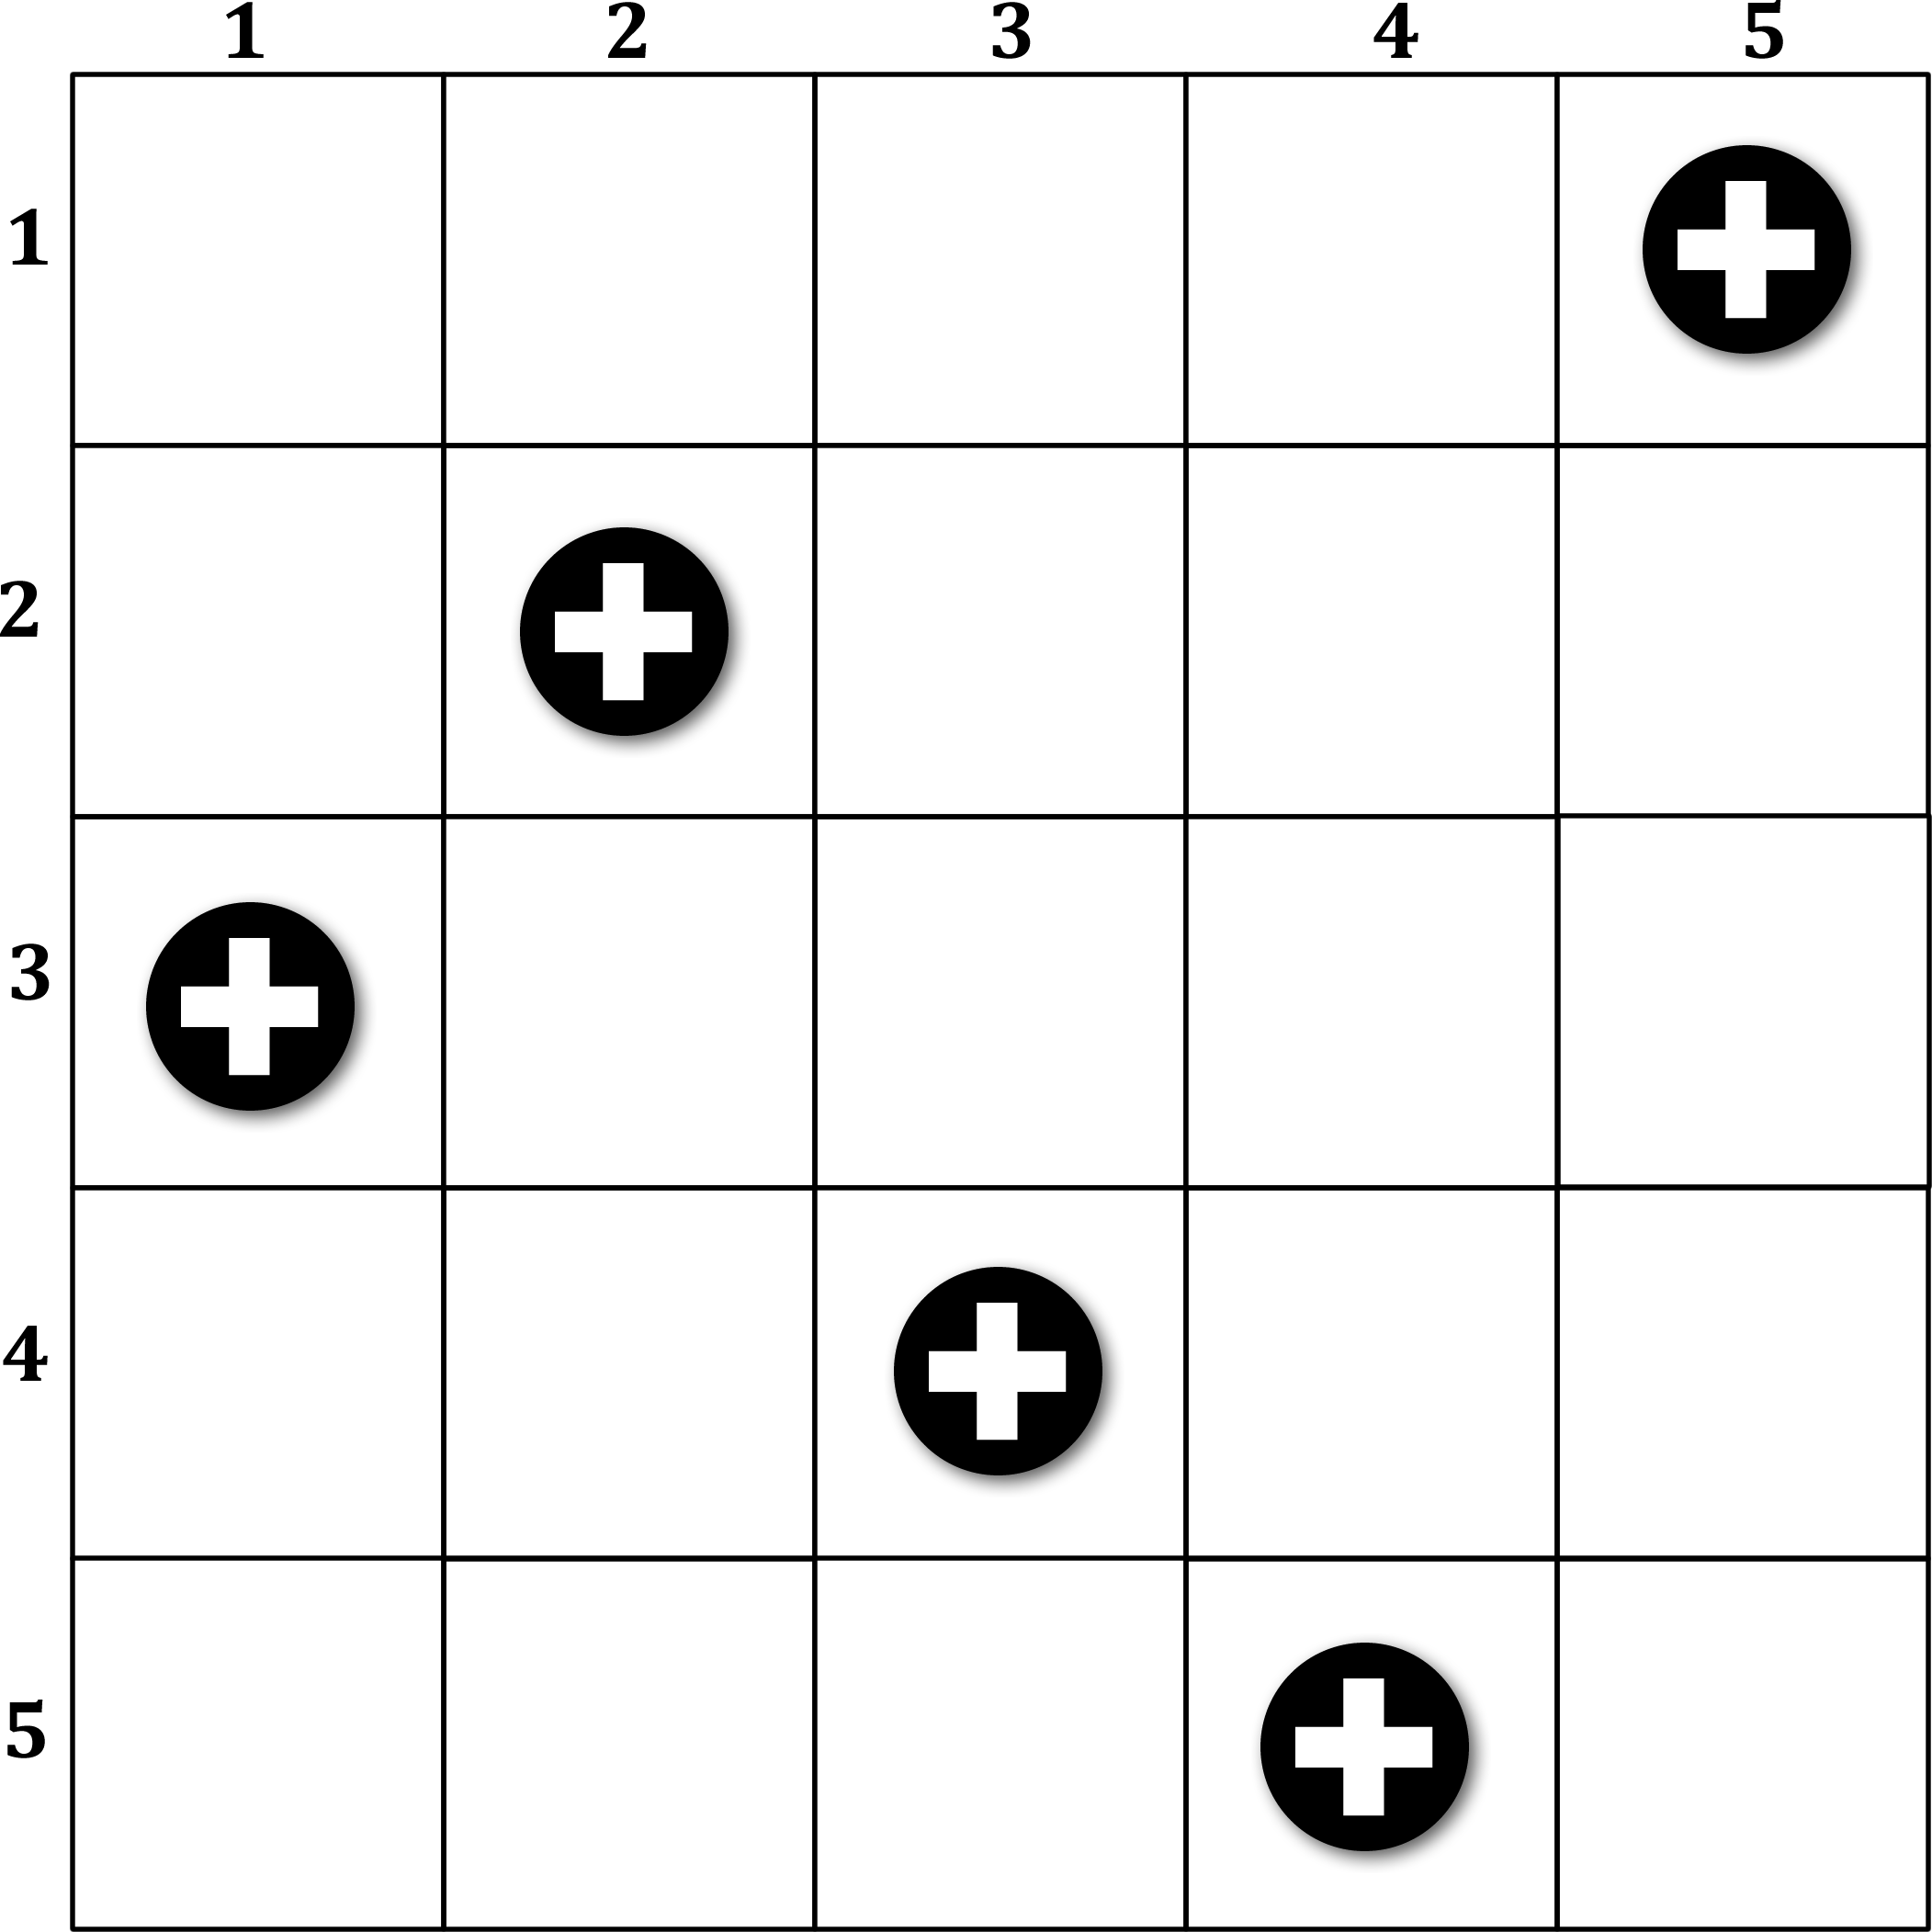
\includegraphics[width=0.35\linewidth]{costas.png}
\caption[]{Example of marks for \CARRP}
\label{fig:ex_costas}
\end{figure}

\new{The cost of the configuration $s$ is then the number of equal elements on each row $d_i$ of its corresponding differences triangle. It can be easily proved that this differences triangle is only necessary to be verified until the row $d_B$, with $B=\floor*{(n-1)/2}$.}

\subsection{Experiments design and results}

To handle this problem, I have reused all modules used for solving the \nqp. First attempts to solve this problems were using the same strategies (\ass) used to solve the \sgp{} and \nqp, without success: \posl{} was not able to solve instances larger than $n = 8$ in a reasonable amount of time (seconds). After many unsuccessful attempts to find the right parameters of \textit{maximum number of restarts}, \textit{maximum number of iterations}, and \textit{maximum number of iterations with the same cost}, I decided to implement the mechanism used by Daniel D\'iaz in the current implementation of {\it Adaptive Search} to escape from local minima: I have added a {\it Reset} \om{} $R_{AS}$ based on the abstract \om{} $R$. The other \oms{} were the same used for solving the \nqp.

Given a configuration $s$, the basic principle of the reset is build another following four steps:
\begin{enumerate}
\item A configuration is obtained by performing left/right shifts to all sub-vectors of $s$ starting or ending by the variable which contributes the most to the cost, and selecting the configuration with the lowest cost.
\item A configurations is obtained by adding a constant (circularly) to each element in the configuration $s$.
\item A configuration is obtained by shifting left from the beginning of $s$ to some culprit variable (i.e. a variable contributing to the cost).
\item Then, one of these 3 generated configuration has the same probability of being selected, to be the result of the reset algorithm. In that sense, some different resets can be performed for the same configuration.
\end{enumerate}


The basic solver used to solve this problem is presented in Algorithm~\ref{as:costas}, and it was taken as a base to build all the different communication strategies. Basically, it is a classical local search iteration, where instead of performing restarts, it performs resets. After a deep analysis of this implementation and results of some runs, I decided to use $K_1 = 2,000,000$ (maximum number of iterations) big enough to solve the chosen instance $n = 19$; and $K_2 = 3$ (the number of iteration before performing the next \textit{reset}).

\begin{algorithm}[H]
\dontprintsemicolon
\SetNoline
\SetKwProg{myproc}{\tet{\bf abstract solver}}{\tet{\bf begin}}{\tet{\bf end}}
\myproc{as\_hard \tcp*{{\sc Itr} $\rightarrow$ number of iterations}
	\tet{\bf computation} : $I, R, V, S, A$\;}{ %\tcp*{{\sc Sci} $\rightarrow$ number of iterations with the same cost}}{%
	$I \poslop{\mapsto}$
	\whileinline{$\left(\textbf{\Iter < } K_1\right)$}{
		$R \poslop{\mapsto}$ % \left[\circlearrowleft (\text{\Iter}\% K_2) \left\{ M_V \longmapsto M_{\hat{S}} \longmapsto M_D\right\}\right]$\;
		\whileinline{$\left(\textbf{\Iter \% } K_2\right)$}{$\left[V \poslop{\mapsto} S \poslop{\mapsto} A\right]$}
	}
}
\tet{\bf solver} \solverposl{single} \tet{\bf implements} as\_hard\;
\algoindent \tet{\bf computation} : $I_{perm},  R_{AS}, V_{AS}, S_{first}, A_{AI}$ \;
%\tet{\bf connection}: $CM_{last}$\;
\caption{Reset-based \as{} for \CARRP}\label{as:costas}
\end{algorithm}

Table~\ref{tab:costas19} shows results of launching \sosets{} to solve each instance of \carrp{} 19 sequentially and in parallel without communication. Runtimes and iteration means showed in this confirm once again the success of the parallel approach. 

\begin{table}[h]
\captionsetup{belowskip=6pt,aboveskip=6pt}
\centering
\renewcommand{\arraystretch}{1}
\begin{tabular}{p{3.5cm}|R{1.5cm}R{1cm}R{1.7cm}R{1.7cm}R{2cm}}
	\hline
	{\bf STRATEGY} & T & T(ds) & It. & It.(sd) & \% success\\
	\hline
	%\hline
	Sequential (1 core) & 132.73 & 80.32 & 2,332,088 & 1,424,757 & 40.00\\
	Parallel (40 cores) & 25.51 & 15.75 & 231,262 & 143,789 & 100.00\\
	\hline
\end{tabular}
\caption{\carr{} 19: no communication}
\label{tab:costas19}
\end{table}

\separation

In order to improve results, a simple communication strategy was applied: communicating the current configuration to other solvers. To do so, we insert a \textit{sending output} operator to the \as{} in Algorithm~\ref{as:costas}. This results in the sender solver presented in Algorithm~\ref{as:costas_sender}. %\tet{et le receiver??? Flo: c'est l'algo 4}

\begin{algorithm}[h]
\dontprintsemicolon
\SetNoline
\SetKwProg{myproc}{\tet{\bf abstract solver}}{\tet{\bf begin}}{\tet{\bf end}}
\myproc{as\_hard\_sender \; %\hspace{3pt}
	\tet{\bf computation} : $I, R, V, S, A$\;}{
	$I \poslop{\mapsto}$
	\whileinline{$\left(\textbf{\Iter} < K_1\right)$}{
		$T \poslop{\mapsto}$
		\whileinline{$\left(\textbf{\Iter \% } K_2\right)$}{$\left[V \poslop{\mapsto} S \poslop{\mapsto} \llparenthesis A \rrparenthesis^d\right]$}
	}
}
\tet{\bf solver} \solverposl{sender} \tet{\bf implements} as\_hard\_sender\;
\algoindent \tet{\bf computation} : $I_{perm}, R_{AS}, V_{AS}, S_{first}, A_{AI}$ \;
%\tet{\bf connection}: $CM_{last}$\;
\caption{Sender solver for \CARRP}\label{as:costas_sender}
\end{algorithm}

Studying some runs of \posl{} solving \CARRP{}, it was observed that \new{during the search process, the cost of the current configuration of all solvers describes an oscillatory descent due to the repeated resets ($K_2 = 3$ in Algorithm~\ref{as:costas}). It means that the cost of the current configuration decreases during $K_2$ iterations and then the current configuration is created by performing a reset which generates generally a more costly configuration. However, in every performed experiment (more than 20 runs with 20 solvers in parallel without communication), the current configuration's cost of the winner solver (first solver finding a solution) described an oscillatory descent also, but not so pronounced (i.e. the difference between the cost of the last current configuration before performing the reset and the cost of the configuration after the reset is not high).} For that reason, it was decided to apply a simple \commstr{} that shares the current configuration while applying the acceptance criterion. To do so, a \opch{} using a \textit{minimum} operator $\poslop{m}$ together with the abstract \om{} $A$ was inserted, as shown in Algorithm~\ref{as:costas_receiver_a}.

One of the main purpose of this study is to explore different communication strategies. We have then implemented and tested different variations of the strategy exposed above by combining two communication operators (\oneTone{} and \oneTn) and different percentages of communicating solvers.
For this problem, it was study also the behavior of the communication performed at two different moments: while applying the acceptance criteria (Algorithm~\ref{as:costas_receiver_a}), and while performing a {\it reset} (Algorithm~\ref{as:costas_receiver_b}).

\begin{algorithm}[h]
\dontprintsemicolon
\SetNoline
\SetKwProg{myproc}{\tet{\bf abstract solver}}{\tet{\bf begin}}{\tet{\bf end}}
\myproc{as\_hard\_receiver\_a \tcp*{{\sc Itr} $\rightarrow$ number of iterations}
	\tet{\bf computation} : $I, T, V, S, A$ \; %\hspace{3pt}
	\tet{\bf communication} : $C.M.$\;}{ 
	$I \poslop{\mapsto}$
	\whileinline{$\left(\textbf{\Iter} < K_1\right)$}{
		$T \poslop{\mapsto}$
		\whileinline{$\left(\textbf{\Iter \% } K_2\right)$}{$\left[V \poslop{\mapsto} S \poslop{\mapsto} \left[A\poslop{m}C.M.\right]\right]$}
	}
}
\tet{\bf solver} \solverposl{receiverA} \tet{\bf implements} as\_hard\_receiver\_a\;
\algoindent\tet{\bf computation} : $I_{perm}, R_{AS}, V_{AS}, S_{first}, A_{AI}$ \; 
\algoindent\tet{\bf communication}: $CM_{last}$\;
\caption{Receiver solver for \CARRP{} (variant A)}\label{as:costas_receiver_a}
\end{algorithm}

\begin{algorithm}[h]
\dontprintsemicolon
\SetNoline
\SetKwProg{myproc}{\tet{\bf abstract solver}}{\tet{\bf begin}}{\tet{\bf end}}
\myproc{as\_hard\_receiver\_b \tcp*{{\sc Itr} $\rightarrow$ number of iterations}
	\tet{\bf computation} : $I, R, V, S, A$\; %\tcp*{{\sc Sci} $\rightarrow$ number of iterations with the same cost}
	\tet{\bf communication} : $C.M.$\;}{%
	$I \poslop{\mapsto}$
	\whileinline{$\left(\textbf{\Iter < } K_1\right)$}{
		$\left[R \poslop{m} C.M.\right] \poslop{\mapsto}$
		\whileinline{$\left(\textbf{\Iter \% } K_2\right)$}{$\left[V \poslop{\mapsto} S \poslop{\mapsto} A\right]$}
	}
}
\tet{\bf solver} \solverposl{receiverB} \tet{\bf implements} as\_hard\_receiver\_b\;
\algoindent\tet{\bf computation} : $I_{perm}, R_{AS}, V_{AS}, S_{first}, A_{AI}$ \; 
\algoindent\tet{\bf connection}: $CM_{last}$\;
\caption{Receiver solver for \CARRP{} (variant B)}\label{as:costas_receiver_b}
\end{algorithm}

The instantiation for receiver solvers instantiates the abstract \opch{} $C.M.$ with the concrete \opch{} $CM_{last}$, which takes into account the last received configuration at the time of its execution.

\begin{table}
\centering 
\renewcommand{\arraystretch}{1}
\resizebox{\columnwidth}{!}{%
\begin{tabular}{p{2.5cm}|R{1.1cm}R{1cm}R{1.3cm}R{1.3cm}|R{1cm}R{1cm}R{1.3cm}R{1.3cm}}
	\hline
	\multirow{3}{*}{\footnotesize{\centering {\bf STRATEGY}}} & \multicolumn{4}{c}{100\% COMM} & \multicolumn{4}{c}{50\% COMM} \\
	\cline{2-9}
	& T & T(sd) & It. & It.(sd) & T & T(sd) & It. & It.(sd)\\
	\hline
	Str A: 1 to 1 & 11.60 & 9.17 & 84,159 & 68,958 & 16.78 & 13.43 & 148,222 & 121,688 \\
	Str A: 1 to N & \good{10.83} & 8.72 & 79,551 & 63,785 & 13.03 & 13.46 & 106,826 & 120,894 \\	
	Str B: 1 to 1 & 14.84 & 13.54 & 119,635 & 112,085 & 14.51 & 13.88 & 125,982 & 123,261 \\
	Str B: 1 to N & 22.99 & 23.82 & 199,930 & 207,851 & 16.62 & 15.16 & 138,840 & 116,858 \\
	\hline
\end{tabular}
}
\caption{\carr{} 19: with communication}
\label{tab:costas19comm}
\end{table}

Table~\ref{tab:costas19comm} shows that \sosets{} executing the strategy {\it A} (receiving the configuration at the time of applying the acceptance criteria) are more effective. \new{The main reason is because in the \commstr{} {\it B}, the communication interferes with the proper performance of the {\it reset}, which is a very important step in the algorithm. Furthermore, the reset provides a very important exploratory factor: when receivers solvers receive the sent configurations and it is accepted by them, they can performed different resets with the same configuration, as it was explained before.}
 
By analyzing the whole information obtained during the experiments, we can observe that the percentage of communicating solvers finding the solution thanks to the received information was high (74\%, see Appendix~\ref{app:cap}, Figure~\ref{barplot:19}). That shows that the communicated information was very helpful during the search process. 
With the simplicity of the operator-based language provided by \posl{}, we were able to find a simple \commstr{} to obtain better results than applying sequential and parallel independent multi-walk approaches. 

\new{Algorithm~\ref{comm:costas1001N} shows the code for the \commstr{} of 100\% of communicating solvers using the \oneTn{} operator $\oneton$. %, where  20 is used as  \textit{syntactic sugar} to declare easily a list of 20 solvers of each type (20 senders and 20 receivers). 
As expected, this was the best \commstr{}. It finds a proper equilibrium between intensification, by communicating a promising place (configuration) inside the search space to a maximum of solvers; and exploration, by performing stochastic decisions once the configuration is accepted, e.g. the must culprit variable is randomly selected if there are more than one, and the way the reset select the returned configuration (explained before).}
%(a good compromise between local computation and data exchange/a fully based communication/ etc) 

\begin{algorithm}
\dontprintsemicolon
\SetNoline
$\left[\eqsolverposl{sender}\posldot A(20)\right] \oneton \left[\eqsolverposl{receiverA}\posldot C.M.(20)\right];$
\caption{Communication strategy \oneTn{} 100\% for \CARRP}\label{comm:costas1001N}
\end{algorithm}

\new{The random nature of this solution strategy has showed to be effective. However, it is the explanation to the high values of standard deviation showe in Table~\ref{tab:costas19comm}. \Ass{} used to the resolution of \CARRP{} combine \oms{} which take many stochastic decisions. The neighborhood \om{} compute the neighborhood based on the most culprit variable of the input configuration, which is randomly selected if there exist more than one. This \m{} also generates neighbors by selecting randomly the variables to swap. In addiction, the reset \om{} generates configurations in three different ways and equally probable, for a same input configuration.}

%\begin{algorithm}[H]
%\dontprintsemicolon
%\SetNoline
%\SetKwProg{myproc}{\tet{\bf abstract solver}}{\tet{\bf begin}}{\tet{\bf end}}
%\myproc{as\_hard\_receiver\_a \tcp*{{\sc Itr} $\rightarrow$ number of iterations}
%	\tet{\bf computation} : $I, R, V, S, A$\; %\tcp*{{\sc Sci} $\rightarrow$ number of iterations with the same cost}
%	\tet{\bf communication} : $C.M.$\;}{%
%	$I \poslop{\mapsto}$\\
%	\While{$\left(\textbf{\Iter < } K_1\right)$}{
%		$R \poslop{\mapsto}$
%		\whileinline{$\left(\textbf{\Iter \% } K_2\right)$}{$\left[V \poslop{\mapsto} S \poslop{\mapsto} \left[A \poslop{m} C.M.\right]\right]$}
%	}
%}
%\caption{Reset-based \as{} for \CARRP{} (receiver, variant A)}\label{as:costas_receiver_a}
%\end{algorithm}
%
%
%\begin{algorithm}[H]
%\dontprintsemicolon
%\SetNoline
%\SetKwProg{myproc}{\tet{\bf abstract solver}}{\tet{\bf begin}}{\tet{\bf end}}
%\myproc{as\_hard\_receiver\_c \tcp*{{\sc Itr} $\rightarrow$ number of iterations}
%	\tet{\bf computation} : $I, R, V, S, A$\; %\tcp*{{\sc Sci} $\rightarrow$ number of iterations with the same cost}
%	\tet{\bf communication} : $C.M.$\;}{%
%	$I \poslop{\mapsto}$\\
%	\While{$\left(\textbf{\Iter < } K_1\right)$}{
%		$\left[R \poslop{m} C.M.\right] \poslop{\mapsto}$
%		\whileinline{$\left(\textbf{\Iter \% } K_2\right)$}{$\left[V \poslop{\mapsto} S \poslop{\mapsto} A\right]$}
%	}
%}
%\caption{Reset-based \as{} for \CARRP{} (receiver, variant C)}\label{as:costas_receiver_c}
%\end{algorithm}